\documentclass[10pt,twocolumn,letterpaper]{article}

\usepackage{statcourse}
\usepackage{times}
\usepackage{epsfig}
\usepackage{graphicx}
\usepackage{amsmath}
\usepackage{amssymb}

% Include other packages here, before hyperref.

% If you comment hyperref and then uncomment it, you should delete
% egpaper.aux before re-running latex.  (Or just hit 'q' on the first latex
% run, let it finish, and you should be clear).
\usepackage[breaklinks=true,bookmarks=false]{hyperref}


\statcoursefinalcopy


\setcounter{page}{1}
\begin{document}


%%%%%%%%%%%%%%%%%%%%%%%%%%%%%%%%%%%%%%%%%%%%%%%%%%%%%%%%%%%%%%%
% DO NOT EDIT ANYTHING ABOVE THIS LINE
% EXCEPT IF YOU LIKE TO USE ADDITIONAL PACKAGES
%%%%%%%%%%%%%%%%%%%%%%%%%%%%%%%%%%%%%%%%%%%%%%%%%%%%%%%%%%%%%%%



%%%%%%%%% TITLE
\title{\LaTeX\ Template for Project Report (\textit{replace with your project title})}

\author{First Author\\
{\tt\small firstauthor@wisc.edu}
\and
Second Author\\
{\tt\small secondauthor@wisc.edu}
\and
Third Author\\
{\tt\small thirdauthor@wisc.edu}
}

\maketitle
%\thispagestyle{empty}



% MAIN ARTICLE GOES BELOW
%%%%%%%%%%%%%%%%%%%%%%%%%%%%%%%%%%%%%%%%%%%%%%%%%%%%%%%%%%%%%%%


%%%%%%%%% ABSTRACT
\begin{abstract}
   The abstract for your project goes here. The length of the abstract
   should be between 200-250 words. Tips for writing a good abstract
   can be found at \url{anonymized}.
\end{abstract}

%%%%%%%%% BODY TEXT

%-------------------------------------------------
\section{Introduction}
%-------------------------------------------------

\noindent\textit{Recommended length: 1/2 to 1 pages.}\vspace{1cm}

For the report, the same rules and guidelines apply as for the proposal. This is an example of a citation \cite{paszke2019pytorch}; if you use the "cite{}" function in LaTeX, the References section will be created automatically at the end of the document. Please read through the {"proposal.pdf"} document for a refresher on how to use citations and figures properly.

Note that the sections for this report are different, and some additional information is contained in this template document, so please read it carefully before you start writing.

This is an example of a mathematical equation:

$$f(\mathbf{x}; \mathbf{w}) = \sum_{i=1}^{n} w_ix_i.$$

This is a mathematical expression, $h(\mathbf{x}) = \hat{y}$ formatted in text. 

The project report should be 6-8 pages long (not counting references)
and should contain the sections that are already provided in this paper. Please
check out the text in these sections for further information.


\subsection{Subsection}

You can use paragraphs or subsections to further structure your
main sections. This is an example of a subsection.

\paragraph{This is a paragraph title.} This is an example of a paragraph.

Ideally, your report should contain all the major sections provided in this report template. Please also consult the "report-rubric.md" for further information on these sections and grading.



%-------------------------------------------------
\section{Related Work}
%-------------------------------------------------

\noindent\textit{Recommended length: 1/2 to 1 pages.}\vspace{1cm}

Related work should be discussed here. This should be a short (1/2 to 1 page) discussion of work (from research papers and articles) that explored similar questions. For example, if you plan to predict COVID-19 from chest X-ray images, discuss previous work that was about a similar project. If the focus of your project is on analyzing the behavior of certain machine learning on a variety of different datasets, and the comparison itself (rather application) is the focus of your paper, discuss other papers that analyzed different algorithms.

%-------------------------------------------------
\section{Proposed Method}
%-------------------------------------------------

\noindent\textit{Recommended length: 1 to 2 pages.}\vspace{1cm}

Describe the method(s) you are proposing, developing, or using. Most students will not propose new or modified machine learning methods or algorithms. In this case, describe how the main algorithms you are using work. This may include mathematical details.

%-------------------------------------------------
\section{Experiments}
%-------------------------------------------------

\noindent\textit{Recommended length: 1/2 to 1 pages.}\vspace{1cm}

Describe the experiments you performed to address specific questions. This includes information about the dataset and software, which are listed as subsections below. Please do not remove these subsections.

\begin{figure}[t]
\begin{center}
   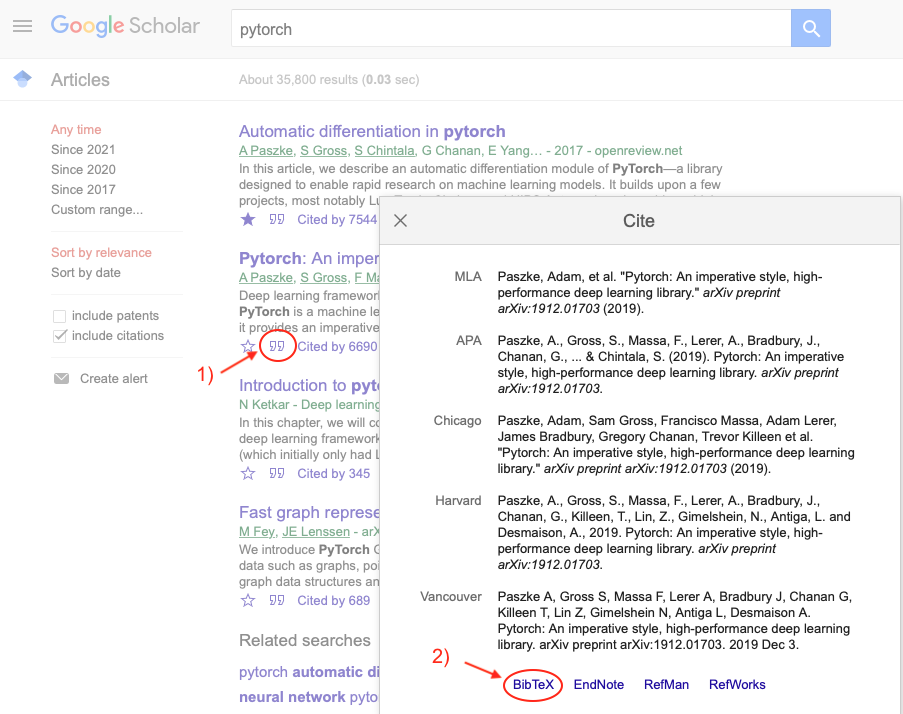
\includegraphics[width=0.8\linewidth]{figures/google-scholar.png}
\end{center}
   \caption{Example of a figure. Please see the {"proposal.pdf"} file for a refresher on using 1-column and 2-column figures.}
\label{fig:google-scholar-1col}
\end{figure}

\subsection{Dataset}

Briefly describe your dataset in a separate subsection.


Table \ref{tab:some-table} shows an example for formatting a table.

\begin{table}
\begin{center}
\begin{tabular}{|l|c|}
\hline
Method & Accuracy \\
\hline\hline
Method 1 & $70 \pm 3$ \% \\
 Method 2 & $76 \pm 3$ \% \\
\hline
\end{tabular}
\end{center}
\label{tab:some-table}
\caption{This is an example of a table.}
\end{table}




\subsection{Software}

Briefly list (and cite) software software you used.

\subsection{Hardware}

If relevant, list hardware resources you used.

%-------------------------------------------------
\section{Results and Discussion}
%-------------------------------------------------

\noindent\textit{Recommended length: 2 to 3 pages.}\vspace{1cm}

Describe the results you obtained from the experiments and interpret them.
Optionally, you could split "Results and Discussion" into two separate
sections, but it is often easier to present the results and discuss them at the same time. In this section, you will likely want to create several subsections that address your specific research questions. As an example for structuring the Results and Discussion section, you can take a look at the following paper: \url{anonymized}.

%-------------------------------------------------
\section{Conclusions}
%-------------------------------------------------

\noindent\textit{Recommended length: 1/3 to 1/2 page.}\vspace{1cm}

Describe your conclusions here. If there are any future directions, you can
describe them here, or you can create a new section for future directions.

%-------------------------------------------------
\section{Acknowledgements}
%-------------------------------------------------

\noindent\textit{Recommended length: 2-4 sentences.}\vspace{1cm}

List acknowledgements if any. For example, if someone provided you a dataset, or
you used someone else's resources, this is a good place to acknowledge
the help or support you received.

%-------------------------------------------------
\section{Contributions}
%-------------------------------------------------

\noindent\textit{Recommended length: 1/3 to 1/2 page.}\vspace{1cm}

Describe the contributions of each team member who worked on this project.


{\small
\bibliographystyle{ieee}
\bibliography{bibliography.bib}
}

\end{document}
